\subsubsection{Deleting Edge from the Root Node}\label{Subsubsec: Deleting Edge from the Root Node}

We first consider the case when the deleted edge (u, v) belongs to the root node of the SCC tree.
The edge is deleted from the graph held in \textsc{STN}(R) as show in \figureref{\ref{fig:tree_node_r_graph_after_dedge1}}.
As we can see in \figureref{\ref{fig:graph_after_dedge_4_to_1}}, the unreachable nodes A and B are removed from \textsc{STN}(R)
and form their own tree nodes in the SCC tree. The SCC-tree corresponding to label $A$ and $B$ gets separated from $R$ and form 
new SCC-trees with root node $A$ and $B$ respectively. The SCC tree is updated as shown in \figureref{\ref{fig:scc_tree_graph_after_del}}.

\begin{figure}[H]
    \centering
    \begin{subfigure}{0.45\textwidth}
        \centering
        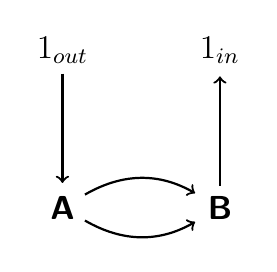
\begin{tikzpicture}[->,shorten >=1pt,auto,node distance=2cm,
            thick,main node/.style={font=\sffamily\large\bfseries}]

        % Define vertices
        \node[main node] (1) {$1_{in}$};
        \node[main node] (11) [left of=1] {$1_{out}$};
        \node[main node] (A) [below of=11] {A};
        \node[main node] (B) [below of=1] {B};
        

        % Draw edges
        \path[every node/.style={font=\sffamily\small}]
            (11) edge (A)
            (A) edge[bend left] (B)
            (A) edge[bend right] (B)
            (B) edge (1);

        \end{tikzpicture}
        \caption{Graph in SCC Tree Node R}
        \label{fig:tree_node_r_graph}
    \end{subfigure}
    \hfill
    \begin{subfigure}{0.45\textwidth}
        \centering
        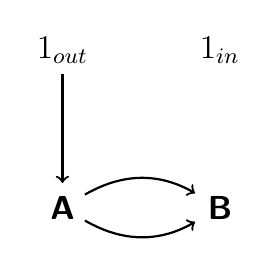
\begin{tikzpicture}[->,shorten >=1pt,auto,node distance=2cm,
            thick,main node/.style={font=\sffamily\large\bfseries}]

        % Define vertices
        \node[main node] (1) {$1_{in}$};
        \node[main node] (11) [left of=1] {$1_{out}$};
        \node[main node] (A) [below of=11] {A};
        \node[main node] (B) [below of=1] {B};
        

        % Draw edges
        \path[every node/.style={font=\sffamily\small}]
            (11) edge (A)
            (A) edge[bend left] (B)
            (A) edge[bend right] (B);

        \end{tikzpicture}
        \caption{Graph after deleting edge 4 to 1}
        \label{fig:graph_after_dedge_4_to_1}
    \end{subfigure}
    \caption{Graph in SCC Tree Node R after deleting edge 4 to 1}
    \label{fig:tree_node_r_graph_after_dedge1}
\end{figure}


\begin{figure}[H]
    \centering
    \begin{subfigure}{0.45\textwidth}
        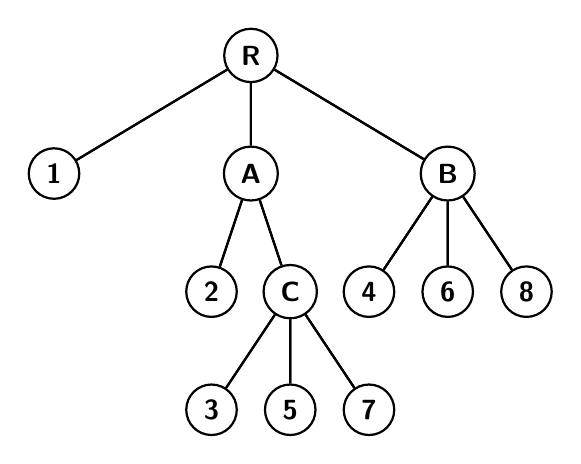
\begin{tikzpicture}[level distance=1.5cm,
                            level 1/.style={sibling distance=2.5cm},
                            level 2/.style={sibling distance=1cm},
                            thick,main node/.style={circle,draw,font=\sffamily\bfseries}]

        % Define vertices
        \node[main node] (R) {R}
            child {node[main node] (1) {1}}
            child {node[main node] (A) {A}
            child {node[main node] (2) {2}}
            child {node[main node] (C) {C}
                child {node[main node] (3) {3}}
                child {node[main node] (5) {5}}
                child {node[main node] (7) {7}}
            }
            }
            child {node[main node] (B) {B}
            child {node[main node] (4) {4}}
            child {node[main node] (6) {6}}
            child {node[main node] (8) {8}}
            };

        % Draw edges
        \path[every node/.style={font=\sffamily\small}]
            (R) edge (1)
            (R) edge (A)
            (R) edge (B)
            (A) edge (2)
            (A) edge (C)
            (B) edge (4)
            (B) edge (6)
            (B) edge (8)
            (C) edge (3)
            (C) edge (5)
            (C) edge (7);

        \end{tikzpicture}
        \caption{SCC Tree of Graph \ref{fig:graph1}}
        \label{fig:scc_tree_graph}
    \end{subfigure}
    \hfill
    \begin{subfigure}{0.5\textwidth}
        \centering
        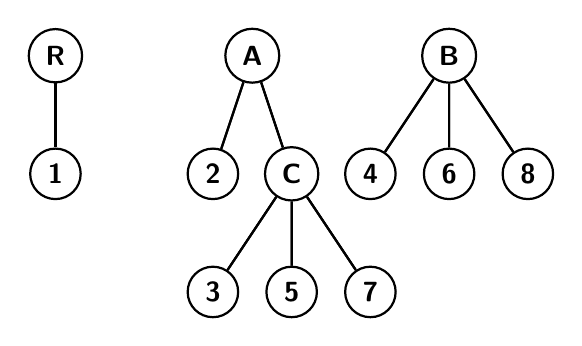
\begin{tikzpicture}[node distance=2.5cm,level distance=1.5cm,
                            level 1/.style={sibling distance=1cm},
                            level 2/.style={sibling distance=1cm},
                            thick,main node/.style={circle,draw,font=\sffamily\bfseries}]

        % Define vertices
        \node[main node] (R) {R}
            child {node[main node] (1) {1}};
        \node[main node] (A) [right of=R] {A}
            child {node[main node] (2) {2}}
            child {node[main node] (C) {C}
                child {node[main node] (3) {3}}
                child {node[main node] (5) {5}}
                child {node[main node] (7) {7}}
            };
        \node[main node] (B) [right of=A] {B}
            child {node[main node] (4) {4}}
            child {node[main node] (6) {6}}
            child {node[main node] (8) {8}};


        % Draw edges
        \path[every node/.style={font=\sffamily\small}]
            (R) edge (1)
            (A) edge (2)
            (A) edge (C)
            (B) edge (4)
            (B) edge (6)
            (B) edge (8)
            (C) edge (3)
            (C) edge (5)
            (C) edge (7);
        \end{tikzpicture}
        \caption{SCC Tree of Graph \ref{fig:graph1} after updates}
        \label{fig:scc_tree_graph_after_del}
    \end{subfigure}
    \caption{SCC Tree updates are propogated, deleting edge 4 to 1}
    \label{fig:scc_tree_after_update_propogation}
\end{figure}

The example in \figureref{\ref{fig:tree_node_r_graph_after_dedge2}} shows the graph in \textsc{STN}(R) after deleting edge 3 to 8. In this case,
the nodes A and B are still reachable and hence remain in the SCC-tree node R. 

\begin{figure}[H]
    \centering
    \begin{subfigure}{0.45\textwidth}
        \centering
        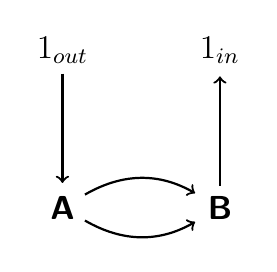
\begin{tikzpicture}[->,shorten >=1pt,auto,node distance=2cm,
            thick,main node/.style={font=\sffamily\large\bfseries}]

        % Define vertices
        \node[main node] (1) {$1_{in}$};
        \node[main node] (11) [left of=1] {$1_{out}$};
        \node[main node] (A) [below of=11] {A};
        \node[main node] (B) [below of=1] {B};
        

        % Draw edges
        \path[every node/.style={font=\sffamily\small}]
            (11) edge (A)
            (A) edge[bend left] (B)
            (A) edge[bend right] (B)
            (B) edge (1);

        \end{tikzpicture}
        \caption{Graph in SCC Tree Node R}
    \end{subfigure}
    \hfill
    \begin{subfigure}{0.45\textwidth}
        \centering
        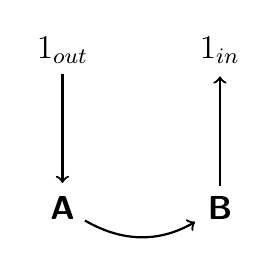
\begin{tikzpicture}[->,shorten >=1pt,auto,node distance=2cm,
            thick,main node/.style={font=\sffamily\large\bfseries}]

        % Define vertices
        \node[main node] (1) {$1_{in}$};
        \node[main node] (11) [left of=1] {$1_{out}$};
        \node[main node] (A) [below of=11] {A};
        \node[main node] (B) [below of=1] {B};
        

        % Draw edges
        \path[every node/.style={font=\sffamily\small}]
            (11) edge (A)
            (A) edge[bend right] (B)
            (B) edge (1);

        \end{tikzpicture}
        \caption{Graph after deleting edge 3 to 8}
        \label{fig:graph_after_dedge_3_to_8}
    \end{subfigure}
    \caption{Graph in SCC Tree Node R after deleting edge 3 to 8}
    \label{fig:tree_node_r_graph_after_dedge2}
\end{figure}